\section{Физическое кодирование}
\subsection{NRZ}
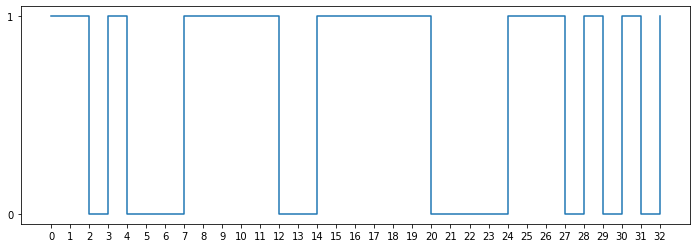
\includegraphics[width=\textwidth]{1nrz}
\begin{center}
    \begin{tabular}{cccc}
        $f_\mathrm{\text{в}}$, МГц & $f_\mathrm{\text{н}}$, МГц & $f_\mathrm{\text{с}}$, МГц & $S$, МГц \\
        500.0 & 62.5 & 214.7 & 3437.5 \\
    \end{tabular}
\end{center}

\subsection{RZ}
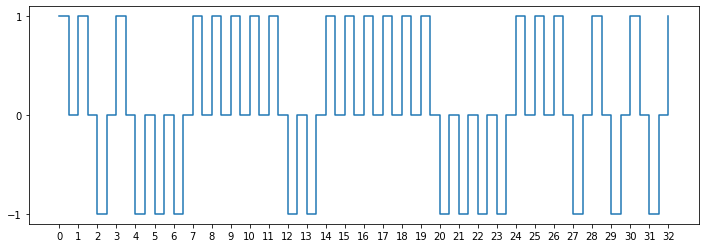
\includegraphics[width=\textwidth]{1rz}
\begin{center}
    \begin{tabular}{cccc}
        $f_\mathrm{\text{в}}$, МГц & $f_\mathrm{\text{н}}$, МГц & $f_\mathrm{\text{с}}$, МГц & $S$, МГц \\
        1000.0 & 500.0 & 994.4 & 6500.0 \\
    \end{tabular}
\end{center}

\subsection{AMI}
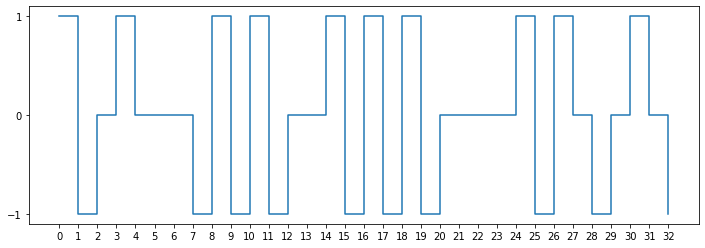
\includegraphics[width=\textwidth]{1ami}
\begin{center}
    \begin{tabular}{cccc}
        $f_\mathrm{\text{в}}$, МГц & $f_\mathrm{\text{н}}$, МГц & $f_\mathrm{\text{с}}$, МГц & $S$, МГц \\
        500.0 & 62.5 & 344.6 & 3437.5 \\
    \end{tabular}
\end{center}

\subsection{NRZI}
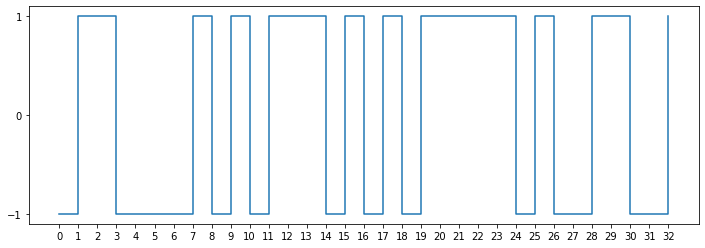
\includegraphics[width=\textwidth]{1nrzi}
\begin{center}
    \begin{tabular}{cccc}
        $f_\mathrm{\text{в}}$, МГц & $f_\mathrm{\text{н}}$, МГц & $f_\mathrm{\text{с}}$, МГц & $S$, МГц \\
        500.0 & 55.6 & 237.3 & 3444.4 \\
    \end{tabular}
\end{center}

\subsection{Манчестерский код}
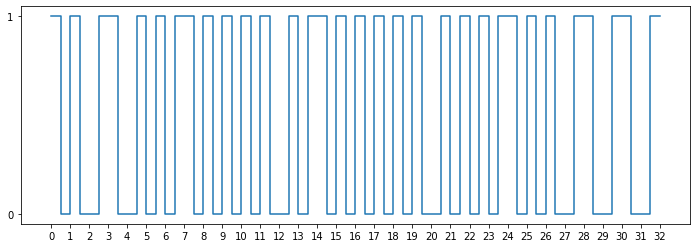
\includegraphics[width=\textwidth]{1manchester}
\begin{center}
    \begin{tabular}{cccc}
        $f_\mathrm{\text{в}}$, МГц & $f_\mathrm{\text{н}}$, МГц & $f_\mathrm{\text{с}}$, МГц & $S$, МГц \\
        1000.0 & 500.0 & 785.3 & 6500.0 \\
    \end{tabular}
\end{center}

\subsection{Дифференциальный манчестерский код}
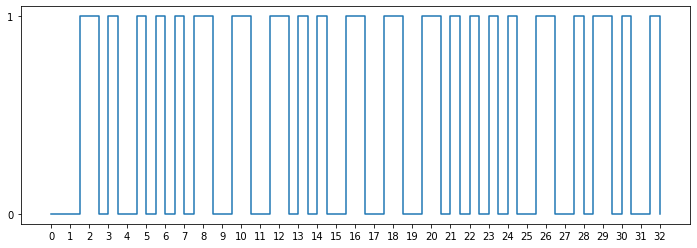
\includegraphics[width=\textwidth]{1manchester_diff}
\begin{center}
    \begin{tabular}{cccc}
        $f_\mathrm{\text{в}}$, МГц & $f_\mathrm{\text{н}}$, МГц & $f_\mathrm{\text{с}}$, МГц & $S$, МГц \\
        1000.0 & 250.0 & 745.9 & 6750.0 \\
    \end{tabular}
\end{center}

\subsection{MLT-3}
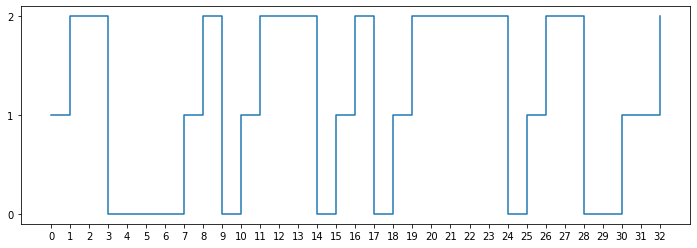
\includegraphics[width=\textwidth]{1mlt3}
\begin{center}
    \begin{tabular}{cccc}
        $f_\mathrm{\text{в}}$, МГц & $f_\mathrm{\text{н}}$, МГц & $f_\mathrm{\text{с}}$, МГц & $S$, МГц \\
        500.0 & 55.6 & 237.3 & 3444.4 \\
    \end{tabular}
\end{center}

\subsection{PAM-5}
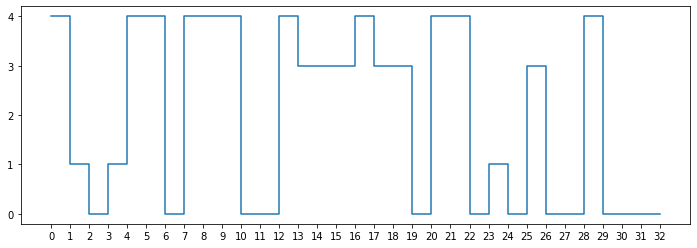
\includegraphics[width=\textwidth]{1pam5}
\begin{center}
    \begin{tabular}{cccc}
        $f_\mathrm{\text{в}}$, МГц & $f_\mathrm{\text{н}}$, МГц & $f_\mathrm{\text{с}}$, МГц & $S$, МГц \\
        500.0 & 125.0 & 348.3 & 3375.0 \\
    \end{tabular}
\end{center}

\subsection{Выбор лучшего}
\begin{center}
    \begin{tabular}{c|cccc}
        & $f_\mathrm{\text{в}}$, МГц
        & $f_\mathrm{\text{н}}$, МГц
        & $f_\mathrm{\text{с}}$, МГц
        & $S$, МГц \\ \hline
        NRZ               &  500.0 &  62.5 & 214.7 & 3437.5 \\
        RZ                & 1000.0 & 500.0 & 994.4 & 6500.0 \\
        AMI               &  500.0 &  62.5 & 344.6 & 3437.5 \\
        NRZI              &  500.0 &  55.6 & 237.3 & 3444.4 \\
        Манчестерский код & 1000.0 & 500.0 & 785.3 & 6500.0 \\
        Дифф. манч. код   & 1000.0 & 250.0 & 745.9 & 6750.0 \\
        MLT-3             &  500.0 &  55.6 & 237.3 & 3444.4 \\
        PAM-5             &  500.0 & 125.0 & 348.3 & 3375.0 \\
    \end{tabular}
\end{center}

\begin{center}
    \begin{tabular}{c|cccc}
        & $S$, МГц
        & Уровни
        & Самосинхронизация
        & Обработка ошибок \\ \hline
        NRZ               & 3437.5 & 2 & - & - \\
        RZ                & 6500.0 & 3 & + & - \\
        AMI               & 3437.5 & 3 & - & + \\
        NRZI              & 3444.4 & 2 & - & - \\
        Манчестерский код & 6500.0 & 2 & + & - \\
        Дифф. манч. код   & 6750.0 & 2 & - & + \\
        MLT-3             & 3444.4 & 3 & - & - \\
        PAM-5             & 3375.0 & 5 & - & + \\
    \end{tabular}
\end{center}

Таким образом, оптимальными являются NRZ и NRZI --- несмотря на отсутствие самосинхронизации,
они обладают наименьшей необходимой полосой пропускания для минимального количества уровней сигнала.
Также хорошим выбором являются обычный и дифференциальный манчестерский код, т.к.
один имеет самосинхронизацию, а другой --- компенсацию ошибок, и оба также имеют лишь 2 уровня сигнала,
но они требуют гораздо более широкой полосы пропускания.

%nrz
%rz
%ami
%nrzi
%manchester
%manchester_diff
%mlt3
%pam5
